%----------------------1----------------------------------------
\begin{frame}[c,plain]{}
    \begin{center}
    Anexos.
    \end{center}
\end{frame}


\begin{frame}[t]{Mapas de interpolación a 20 \textcelsius.}
    \begin{figure}
    \begin{subfigure}[b]{0.45\textwidth}
        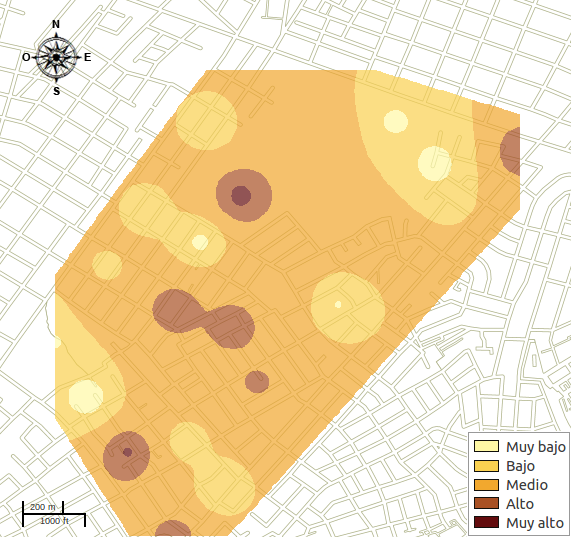
\includegraphics[width=\textwidth]{../book/capitulo-6/graphics/raster/temp-20-0.png}
        \caption{ Primer día de simulación.}
    \end{subfigure}
    ~~~~
    \begin{subfigure}[b]{0.45\textwidth}
        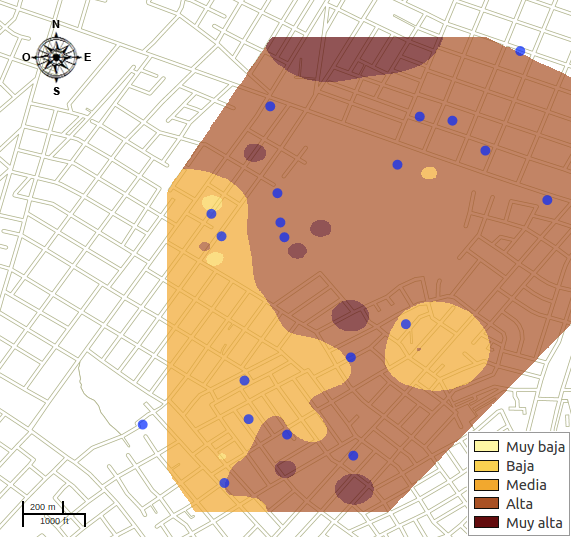
\includegraphics[width=\textwidth]{../book/capitulo-6/graphics/raster/temp-20-38.png}
        \caption{Día número 50 de simulación.}
    \end{subfigure}
    \end{figure}
\end{frame}

\begin{frame}[t]{Mapas de interpolación a 24 \textcelsius.}
    \begin{figure}
    \begin{subfigure}[b]{0.45\textwidth}
        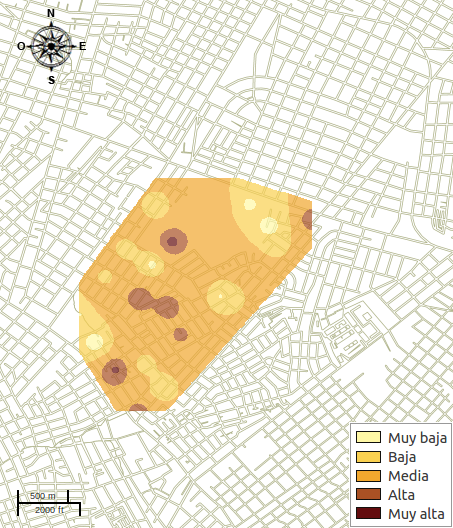
\includegraphics[width=4.5cm]{../book/capitulo-6/graphics/raster/temp-24-0.png}
        \caption{ Primer día de simulación.}
    \end{subfigure}
    ~~~~
    \begin{subfigure}[b]{0.45\textwidth}
        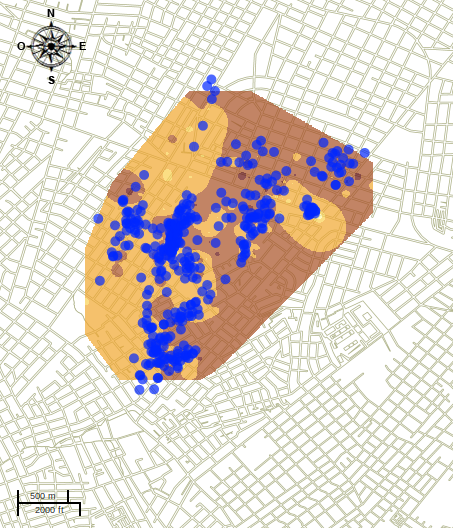
\includegraphics[width=4.5cm]{../book/capitulo-6/graphics/raster/temp-24-49.png}
        \caption{Día número 50 de simulación.}
    \end{subfigure}
    \end{figure}
\end{frame}

\begin{frame}[t]{Mapas de interpolación a 27 \textcelsius.}
    \begin{figure}
    \begin{subfigure}[b]{0.45\textwidth}
        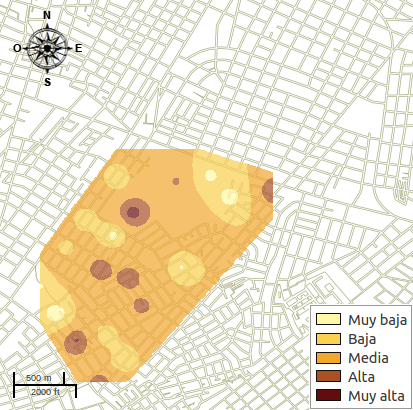
\includegraphics[width=\textwidth]{../book/capitulo-6/graphics/raster/temp-27-0.png}
        \caption{ Primer día de simulación.}
    \end{subfigure}
    ~~~~
    \begin{subfigure}[b]{0.45\textwidth}
        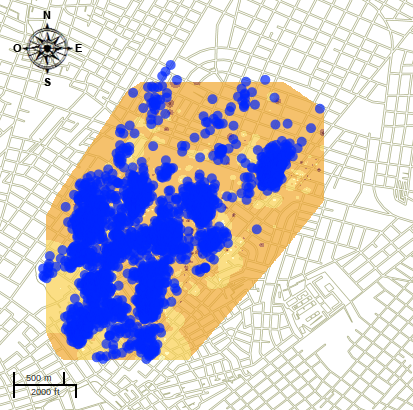
\includegraphics[width=\textwidth]{../book/capitulo-6/graphics/raster/temp-27-49.png}
        \caption{Día número 50 de simulación}
    \end{subfigure}
    \end{figure}
\end{frame}

\begin{frame}[t]{Mapas de interpolación a 34 \textcelsius.}
    \begin{figure}
    \begin{subfigure}[b]{0.45\textwidth}
        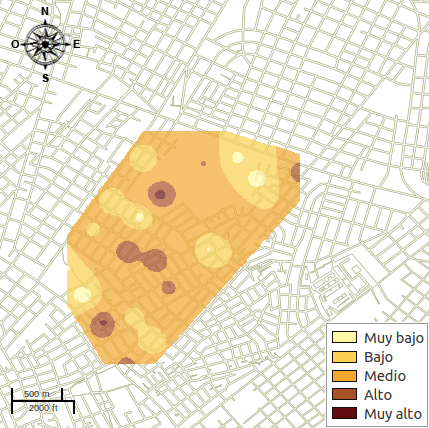
\includegraphics[width=\textwidth]{../book/capitulo-6/graphics/raster/temp-34-0.png}
        \caption{ Primer día de simulación.}
    \end{subfigure}
    ~~~~
    \begin{subfigure}[b]{0.45\textwidth}
        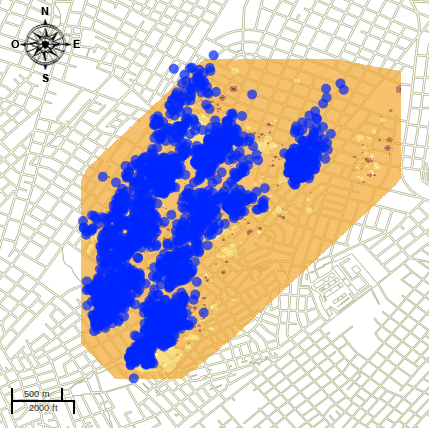
\includegraphics[width=\textwidth]{../book/capitulo-6/graphics/raster/temp-34-42.png}
        \caption{Día número 50 de simulación.}
    \end{subfigure}
    \end{figure}
\end{frame}


\begin{frame}[c]{Ovitrampas.}
  \begin{center}
    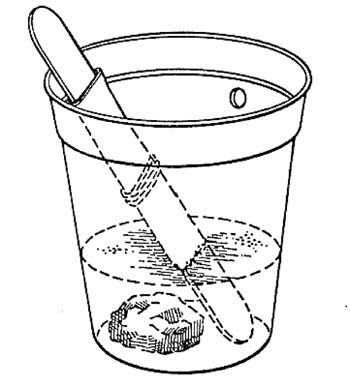
\includegraphics[width=6cm]{../book/capitulo-3/graphics/ovitrampa.jpg}
  \end{center}
\end{frame}

\begin{frame}[c]{Strack tecnológico.}
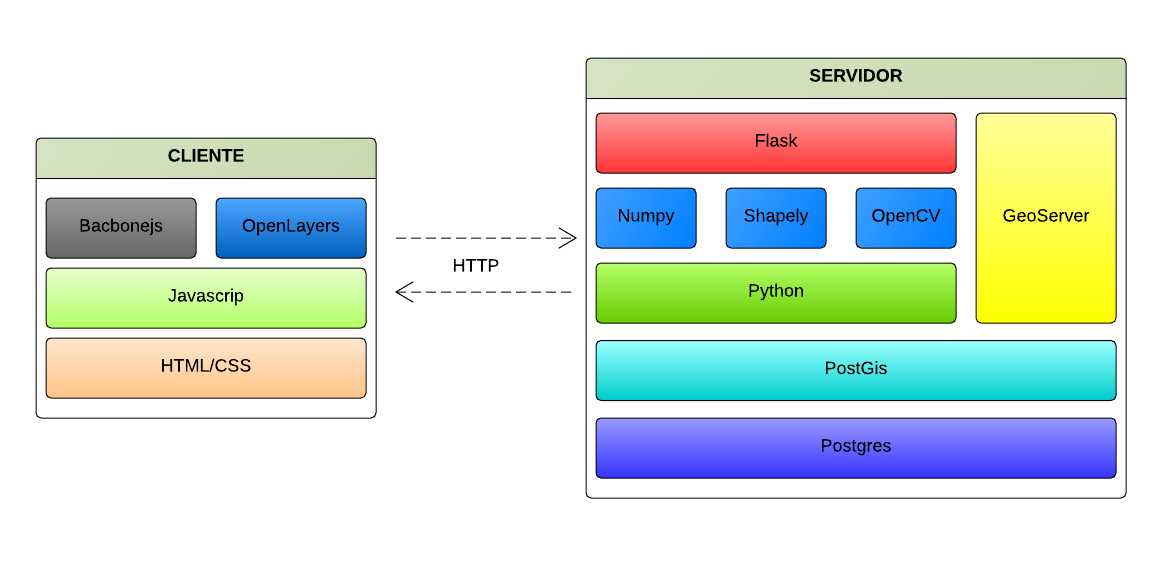
\includegraphics[width=\textwidth]{../book/capitulo-5/graphics/stack-tecnologias.png}
\end{frame}


\begin{frame}[c]{Conteo de larvas con PDI.}
    \begin{figure}
    \begin{subfigure}[b]{0.45\textwidth}
        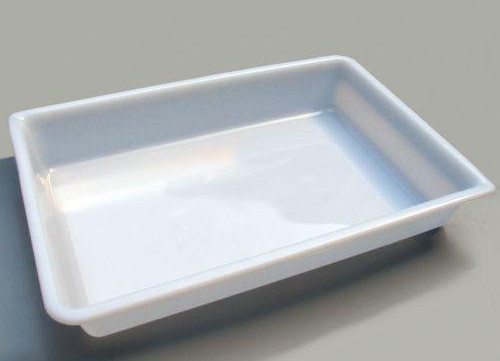
\includegraphics[width=4.5cm]{../book/capitulo-5/graphics/bandeja-muestra.jpg}
        \caption{Bandeja vacía.}
    \end{subfigure}
    ~~~~
    \begin{subfigure}[b]{0.45\textwidth}
        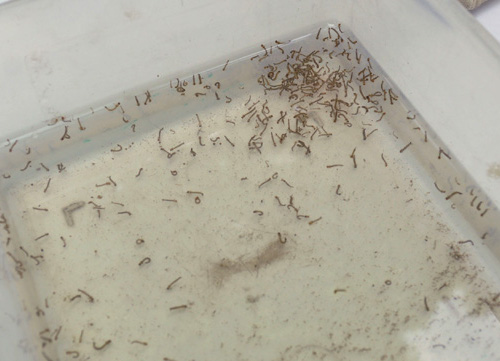
\includegraphics[width=4.5cm]{../book/capitulo-5/graphics/larvas-dengue.jpg}
        \caption{Bandeja con larvas.}
    \end{subfigure}
    \end{figure}
\end{frame}

\begin{frame}[c]{Conteo de larvas con PDI (2).}
    \begin{figure}
    \begin{subfigure}[t]{0.45\textwidth}
        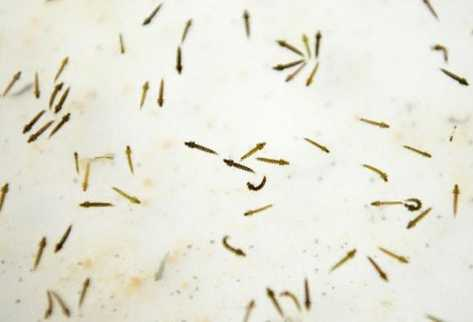
\includegraphics[width=4.5cm]{../book/capitulo-5/graphics/larvas-original.png}
        \caption{Imagen original.}
    \end{subfigure}
    ~~~~
    \begin{subfigure}[t]{0.45\textwidth}
        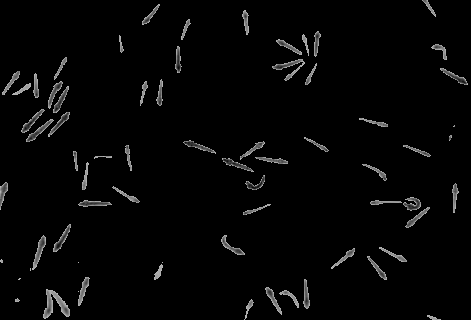
\includegraphics[width=4.5cm]{../book/capitulo-5/graphics/larvas-otsu.png}
        \caption{Imagen luego de la umbralización.}
    \end{subfigure}
    \end{figure}
\end{frame}

\begin{frame}[t]{Coeficientes del modelo de Sharpe y DeMichele.}
\begin{table}
\begin{minipage}{\textwidth}
    \centering
    \small
    \caption{ \label{tab:coef-sharpe-demichele} Coeficientes para el modelo simplificado de Sharpe y DeMichele, con inhibición de altas temperaturas presentado por Schoolfield.}
    \begin{tabular}{l c r r r r }
        \hline \\
        Ciclo de desarrollo    & $R(298K)$ & $\Delta H_{A}$ & $\Delta H_{H}$ & $\Delta T_{1/2}$  \\
        \hline
        \hline
        Eclosión de los huevos$^a$ & 0,24000 & 10798,00 &  100000,00  & 14184,000\\
        Desarrollo larvario$^b$    & 0,20429 & 36072,78 &   59147,51  &   301,560\\
        Desarrollo pupal$^b$       & 0,74423 & 19246,42 &    5954,35  &   302,687\\
        Ciclo gonotrófico (AN)$^c$ & 0,21600 & 15725,00 & 1756481,00  &   447,200\\
        Ciclo gonotrófico (AP)$^c$ & 0,37200 & 15725,00 & 1756481,00  &   447,200\\
    \end{tabular}
    \footnotetext[1]{Coeficientes Otero et al., 2006.}
    \footnotetext[2]{Coeficientes Rueda et al.,1990.}
    \footnotetext[3]{Coeficientes, para AP y AN, tomados Otero et al., 2006.}
\end{minipage}
\end{table}
\end{frame}
